\documentclass[tikz,border=0pt]{standalone}
\usepackage{lipsum} % for sample text
\definecolor{lavender}{HTML}{ced4d9}
\definecolor{bblue}{HTML}{e1e9ef}
\definecolor{lyellow}{HTML}{faf1b6}

\definecolor{green1}{HTML}{c2d3b5}
\definecolor{green2}{HTML}{7ba05e}
\definecolor{red1}{HTML}{e1c1c2}
\definecolor{red2}{HTML}{96474a}
\usepackage{soul}
\usepackage{color}

\DeclareRobustCommand{\hlcyan}[1]{{\sethlcolor{lyellow}\hl{#1}}}
\def\y{0.92}
\begin{document}

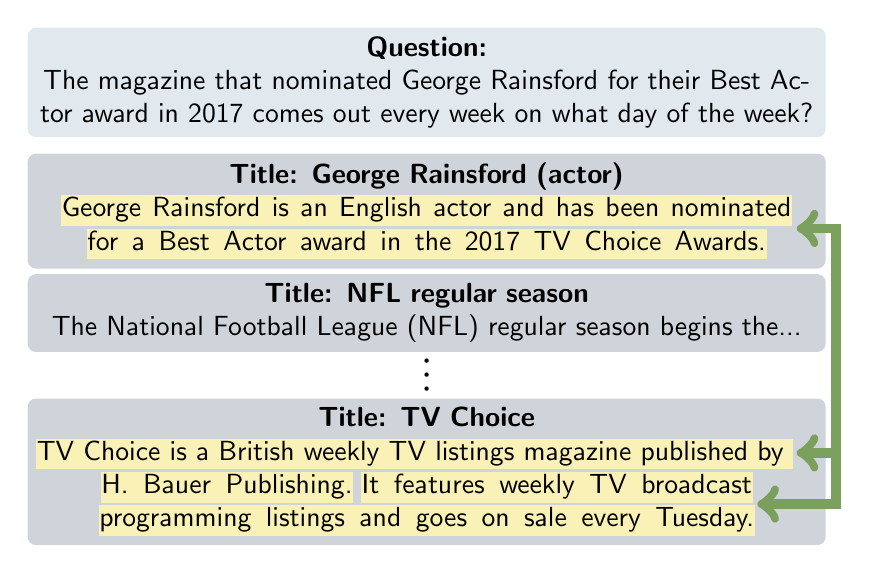
\begin{tikzpicture}

    \node[fill=bblue, text width=9.9cm, align=center, rounded corners=3pt, line width=0,
    font=\sffamily, anchor=north] (node1) at (5.1, 5.7) 
    {\textbf{Question:}\\The magazine that nominated George Rainsford for their Best Actor award in 2017 comes out every week on what day of the week?};
        \node[fill=lavender, text width=9.9cm, align=center, rounded corners=3pt, line width=0,
    font=\sffamily, anchor=north] (node1) at (5.1, 4.1) 
    {\textbf{Title: George Rainsford (actor)}\\\hlcyan{George Rainsford is an English actor and has been nominated for a Best Actor award in the 2017 TV Choice Awards.}};

        \node[fill=lavender, text width=9.9cm, align=center, rounded corners=3pt, line width=0,
    font=\sffamily, anchor=north] (node1) at (5.1, 1.65+\y) 
    {\textbf{Title: NFL regular season}\\The National Football League (NFL) regular season begins the...};
\node[font=\bfseries, rotate=90] at (5.1, 0.4+\y) {\dots};
        \node[fill=lavender, text width=9.9cm, align=center, rounded corners=3pt, line width=0,
    font=\sffamily, anchor=north] (node1) at (5.1, 0.07+\y) 
    {\textbf{Title: TV Choice }\\\hlcyan{TV Choice is a British weekly TV listings magazine published by \\ H. Bauer Publishing.} \hlcyan{It features weekly TV broadcast programming listings and goes on sale every Tuesday.}};;

    \draw[<->, line width=3.5pt, color=green2] (9.3,-.35) -- (10.3,-.35) -- (10.3,3.15) -- (9.8,3.15);
    \draw[<-, line width=3.5pt, color=green2] (9.8,.3) -- (10.3,.3);
    
\end{tikzpicture}

\end{document}